\tocsubsection{Tuần 3}

\tocsubsubsection{3.1 Mô tả công việc}

Trong tuần 3 của kỳ thực tập, sinh viên tập trung nghiên cứu kiến trúc phần mềm cho hệ thống quản lý thiết bị IoT trong dự án SmartWater. Trên cơ sở hồ sơ đề xuất kỹ thuật, các tài liệu nghiệp vụ và quá trình trao đổi với người hướng dẫn, sinh viên tiến hành phân tích bài toán, xác định các yêu cầu của hệ thống và xây dựng mô hình kiến trúc phù hợp trước khi bắt đầu giai đoạn phát triển.

Bên cạnh việc nghiên cứu kiến trúc tổng thể, sinh viên tìm hiểu giao thức MQTT, cơ chế Publish/Subscribe và phương thức kết nối đến HiveMQ Cloud thông qua MQTT over WebSocket. Đồng thời, sinh viên khảo sát luồng dữ liệu từ thiết bị IoT đến hệ thống quản lý nhằm xác định vai trò của từng thành phần trong quá trình thu nhận, xử lý và khai thác dữ liệu telemetry.

Các công việc đã thực hiện trong tuần gồm:

\begin{itemize}
    \item Phân tích bài toán và yêu cầu của hệ thống SmartWater.
    \item Đề xuất và đánh giá các phương án kiến trúc phần mềm.
    \item Thiết kế kiến trúc tổng thể của hệ thống quản lý IoT.
    \item Thiết kế kiến trúc Device Monitor.
    \item Thiết kế kiến trúc SmartWater Admin.
    \item Xây dựng mô hình luồng dữ liệu telemetry.
    \item Khảo sát giao thức MQTT, HiveMQ Cloud và MQTT over WebSocket.
    \item Khảo sát, đánh giá và lựa chọn các công nghệ phục vụ phát triển hệ thống.
\end{itemize}
\tocsubsubsection{3.2 Thiết kế kiến trúc phần mềm}

Sau khi nghiên cứu hồ sơ đề xuất kỹ thuật và xác định phạm vi của dự án, sinh viên tiến hành thiết kế kiến trúc phần mềm cho hệ thống SmartWater. Đây là bước quan trọng nhằm xác định các thành phần của hệ thống, phân chia trách nhiệm giữa các ứng dụng và xây dựng luồng xử lý dữ liệu từ thiết bị IoT đến hệ thống quản lý.

Mục tiêu của giai đoạn này không chỉ là đáp ứng yêu cầu hiện tại của dự án mà còn xây dựng một kiến trúc có khả năng mở rộng, giúp việc bổ sung các chức năng hoặc ứng dụng mới trong tương lai được thực hiện dễ dàng mà không làm ảnh hưởng đến các thành phần đang hoạt động.

Quá trình thiết kế được thực hiện thông qua các bước gồm phân tích bài toán, xác định yêu cầu thiết kế, đánh giá các phương án kiến trúc và đề xuất mô hình kiến trúc phù hợp với đặc điểm của hệ thống.

\tocsubsubsubsection{3.2.1 Phân tích bài toán}

Trước khi tiến hành thiết kế kiến trúc phần mềm, sinh viên thực hiện phân tích bài toán nhằm xác định đặc điểm hoạt động của hệ thống SmartWater, các yêu cầu đặt ra trong quá trình vận hành và những vấn đề cần giải quyết trong quá trình thiết kế.

Hệ thống SmartWater được xây dựng nhằm quản lý các máy lọc nước được triển khai tại nhiều vị trí khác nhau. Mỗi máy lọc nước được trang bị một vi điều khiển (MCU) có nhiệm vụ thu thập dữ liệu từ các cảm biến và định kỳ gửi dữ liệu telemetry lên hệ thống thông qua Internet. Dữ liệu này được sử dụng để theo dõi trạng thái hoạt động của thiết bị, hỗ trợ công tác giám sát và làm cơ sở cho các nghiệp vụ bảo trì.

Qua quá trình khảo sát hồ sơ đề xuất kỹ thuật, sinh viên nhận thấy hệ thống có một số đặc điểm quan trọng sau:

\begin{itemize}
    \item Số lượng thiết bị có thể tăng lên theo quá trình triển khai thực tế, do đó lượng dữ liệu telemetry sẽ tăng tương ứng.

    \item Dữ liệu telemetry được gửi theo chu kỳ và liên tục trong suốt quá trình vận hành của thiết bị.

    \item Hệ thống không chỉ xử lý dữ liệu từ thiết bị mà còn phải đáp ứng các nghiệp vụ quản lý như khách hàng, hợp đồng, máy lọc nước, thiết bị, kho và kế hoạch bảo trì.

    \item Dữ liệu telemetry được nhiều chức năng cùng khai thác, chẳng hạn như hiển thị Dashboard, theo dõi trạng thái thiết bị, lập kế hoạch bảo trì hoặc phục vụ các chức năng phân tích trong tương lai.
\end{itemize}

Từ các đặc điểm trên, sinh viên tiến hành phân loại bài toán thành hai nhóm chức năng chính.

\begin{itemize}
    \item \textbf{Nhóm xử lý dữ liệu IoT}: bao gồm việc tiếp nhận, kiểm tra, xử lý và lưu trữ dữ liệu telemetry từ các thiết bị.

    \item \textbf{Nhóm quản lý nghiệp vụ}: bao gồm các chức năng quản lý khách hàng, hợp đồng, máy lọc nước, thiết bị, kho, bảo trì và hiển thị dữ liệu cho người sử dụng.
\end{itemize}

Hai nhóm chức năng này có mục đích, đặc điểm hoạt động và tải xử lý khác nhau. Trong khi nhóm xử lý dữ liệu IoT yêu cầu hoạt động liên tục để tiếp nhận dữ liệu từ thiết bị, nhóm quản lý nghiệp vụ chỉ phát sinh khi người dùng thực hiện các thao tác trên hệ thống.

Nếu toàn bộ chức năng được triển khai trong cùng một ứng dụng, hệ thống sẽ phải đồng thời xử lý dữ liệu telemetry và các nghiệp vụ quản lý. Điều này làm tăng sự phụ thuộc giữa các thành phần, gây khó khăn trong việc bảo trì, đồng thời hạn chế khả năng mở rộng khi cần bổ sung thêm các chức năng hoặc ứng dụng mới.

Từ kết quả phân tích trên, sinh viên nhận thấy kiến trúc phần mềm cần tách biệt giữa lớp thu nhận dữ liệu và lớp quản lý nghiệp vụ, đồng thời xây dựng một nguồn dữ liệu telemetry dùng chung để nhiều ứng dụng có thể khai thác mà không làm ảnh hưởng lẫn nhau.
\tocsubsubsubsection{3.2.2 Xác định yêu cầu thiết kế}

Từ kết quả phân tích bài toán, sinh viên tiến hành xác định các yêu cầu mà kiến trúc phần mềm cần đáp ứng. Các yêu cầu này được xây dựng dựa trên đặc điểm hoạt động của hệ thống, nhu cầu quản lý thực tế cũng như định hướng phát triển lâu dài của dự án.

Qua quá trình phân tích, sinh viên nhận thấy kiến trúc của hệ thống không chỉ cần đảm bảo khả năng thu nhận dữ liệu từ các thiết bị IoT mà còn phải tạo điều kiện thuận lợi cho việc phát triển, bảo trì và mở rộng các chức năng trong tương lai. Vì vậy, các yêu cầu thiết kế được chia thành bốn nhóm chính như sau.

\paragraph*{(1) Yêu cầu về xử lý dữ liệu}

Kiến trúc cần đảm bảo khả năng tiếp nhận dữ liệu telemetry từ nhiều thiết bị hoạt động đồng thời. Dữ liệu sau khi tiếp nhận phải được kiểm tra, chuẩn hóa và lưu trữ tập trung trước khi được các ứng dụng khác khai thác. Việc chuẩn hóa dữ liệu giúp đảm bảo tính nhất quán giữa các thành phần và tạo điều kiện thuận lợi cho việc tái sử dụng dữ liệu.

\paragraph*{(2) Yêu cầu về phân chia chức năng}

Quá trình thu nhận dữ liệu từ thiết bị và các nghiệp vụ quản lý cần được tách thành các thành phần độc lập. Mỗi thành phần chỉ đảm nhiệm một nhóm chức năng cụ thể nhằm giảm sự phụ thuộc trong hệ thống, đồng thời giúp việc phát triển và bảo trì trở nên đơn giản hơn.

\paragraph*{(3) Yêu cầu về khả năng mở rộng}

Một trong những mục tiêu quan trọng của kiến trúc là hỗ trợ việc mở rộng chức năng của hệ thống. Trong quá trình phát triển, hệ thống có thể được bổ sung thêm các ứng dụng hoặc dịch vụ mới như hệ thống cảnh báo, phân tích dữ liệu, dự đoán bảo trì hoặc các nền tảng quản lý khác mà không cần thay đổi kiến trúc của các thành phần hiện có.

Ngoài việc mở rộng chức năng, từng thành phần cũng cần có khả năng được nâng cấp hoặc thay thế độc lập khi yêu cầu của dự án thay đổi.

\paragraph*{(4) Yêu cầu về khả năng bảo trì}

Kiến trúc cần được tổ chức theo hướng phân chia rõ trách nhiệm giữa các thành phần, giúp mã nguồn dễ quản lý, thuận tiện cho việc kiểm thử, bảo trì và triển khai các phiên bản mới. Đồng thời, việc giảm sự phụ thuộc giữa các thành phần sẽ hạn chế ảnh hưởng dây chuyền khi thực hiện thay đổi hoặc bổ sung chức năng.

\tocsubsubsubsection{3.2.3 Đề xuất giải pháp kiến trúc}

Sau khi xác định các yêu cầu thiết kế, sinh viên tiến hành nghiên cứu và đánh giá các phương án kiến trúc nhằm lựa chọn mô hình phù hợp với đặc điểm của hệ thống SmartWater. Việc lựa chọn kiến trúc không chỉ cần đáp ứng các yêu cầu hiện tại mà còn phải đảm bảo khả năng phát triển lâu dài của dự án.

Để đánh giá các phương án, sinh viên sử dụng một số tiêu chí chính sau:

\begin{itemize}
    \item Khả năng đáp ứng yêu cầu xử lý dữ liệu telemetry từ các thiết bị IoT.
    \item Mức độ phân tách giữa lớp xử lý dữ liệu và lớp nghiệp vụ.
    \item Khả năng mở rộng chức năng của hệ thống trong tương lai.
    \item Khả năng bảo trì và nâng cấp từng thành phần.
    \item Mức độ phụ thuộc giữa các module trong hệ thống.
\end{itemize}

% Dựa trên các tiêu chí trên, sinh viên tiến hành phân tích hai phương án triển khai.

% \paragraph*{Phương án 1: Hệ thống đơn khối (Monolithic Application)}

% Ở phương án này, toàn bộ chức năng của hệ thống được triển khai trong một ứng dụng duy nhất. Ứng dụng vừa thực hiện kết nối đến MQTT Broker, tiếp nhận và xử lý dữ liệu telemetry, vừa đảm nhiệm các nghiệp vụ quản lý như khách hàng, hợp đồng, thiết bị và bảo trì.

% Ưu điểm của phương án này là kiến trúc tương đối đơn giản, quá trình triển khai ban đầu nhanh và việc trao đổi dữ liệu giữa các module diễn ra trực tiếp trong cùng một ứng dụng.

% Tuy nhiên, khi quy mô hệ thống tăng lên, toàn bộ các chức năng đều tập trung trong một mã nguồn sẽ làm tăng mức độ phụ thuộc giữa các module. Mọi thay đổi trong quá trình xử lý telemetry đều có thể ảnh hưởng đến các nghiệp vụ quản lý và ngược lại. Ngoài ra, khi cần bổ sung các chức năng mới hoặc phát triển thêm các ứng dụng khác, việc tái sử dụng dữ liệu và mở rộng hệ thống sẽ gặp nhiều khó khăn.
    

% \paragraph*{Phương án 2: Kiến trúc phân tách theo chức năng (Microservice)}

% Ở phương án này, hệ thống được chia thành các thành phần độc lập, mỗi thành phần đảm nhiệm một nhóm chức năng riêng biệt.

% MQTT Broker chịu trách nhiệm truyền nhận dữ liệu giữa các thiết bị IoT và hệ thống. Device Monitor đóng vai trò tiếp nhận dữ liệu telemetry, thực hiện kiểm tra, chuẩn hóa và lưu trữ dữ liệu vào cơ sở dữ liệu telemetry. SmartWater Admin tập trung vào các nghiệp vụ quản lý và khai thác dữ liệu đã được xử lý để phục vụ việc giám sát và vận hành hệ thống.

% Việc phân chia theo chức năng giúp tách biệt rõ ràng giữa lớp thu nhận dữ liệu và lớp quản lý nghiệp vụ. Mỗi thành phần có thể được phát triển, kiểm thử và triển khai độc lập mà không ảnh hưởng đến các thành phần còn lại. Đồng thời, dữ liệu telemetry sau khi được chuẩn hóa có thể được sử dụng bởi nhiều ứng dụng khác nhau thay vì chỉ phục vụ SmartWater Admin.



% Từ kết quả phân tích, sinh viên đề xuất kiến trúc phần mềm gồm các thành phần chính là thiết bị IoT, MQTT Broker, Device Monitor, cơ sở dữ liệu telemetry và SmartWater Admin.

% Trong mô hình này, các thiết bị IoT đóng vai trò thu thập dữ liệu từ cảm biến và định kỳ gửi dữ liệu telemetry lên MQTT Broker theo cơ chế Publish/Subscribe. Device Monitor kết nối đến MQTT Broker thông qua MQTT over WebSocket để tiếp nhận các bản tin, kiểm tra tính hợp lệ của dữ liệu, chuẩn hóa cấu trúc dữ liệu và bổ sung các thông tin cần thiết trước khi lưu vào cơ sở dữ liệu telemetry.

% SmartWater Admin không giao tiếp trực tiếp với MQTT Broker mà sử dụng dữ liệu telemetry đã được Device Monitor xử lý kết hợp với dữ liệu nghiệp vụ để phục vụ các chức năng quản lý khách hàng, hợp đồng, máy lọc nước, thiết bị và bảo trì.

% Kiến trúc này tạo ra sự tách biệt giữa lớp thu nhận dữ liệu và lớp quản lý nghiệp vụ, đồng thời hình thành một nguồn dữ liệu telemetry dùng chung để các ứng dụng khác có thể khai thác trong tương lai.

% Hình \ref{fig:software-architecture} mô tả kiến trúc phần mềm được đề xuất.


\tocsubsubsubsection{3.2.5 Đánh giá và lựa chọn kiến trúc phù hợp}

% Sau khi phân tích hai phương án kiến trúc, sinh viên tiến hành đánh giá mức độ phù hợp của từng phương án dựa trên các tiêu chí về khả năng mở rộng, tính độc lập giữa các thành phần, khả năng bảo trì và định hướng phát triển lâu dài của hệ thống.

% Đối với phương án hệ thống đơn khối, toàn bộ chức năng từ tiếp nhận dữ liệu MQTT, xử lý telemetry đến quản lý nghiệp vụ đều được triển khai trong cùng một ứng dụng. Mặc dù phương án này giúp đơn giản hóa quá trình phát triển ở giai đoạn đầu, nhưng khi số lượng thiết bị hoặc chức năng tăng lên, ứng dụng sẽ phải xử lý đồng thời nhiều loại tác vụ khác nhau. Điều này làm tăng mức độ phụ thuộc giữa các module và gây khó khăn khi cần bảo trì hoặc mở rộng hệ thống.

% Hình \ref{fig:monolithic} minh họa kiến trúc đơn khối của hệ thống.

% \begin{figure}[H]
%     \centering
%     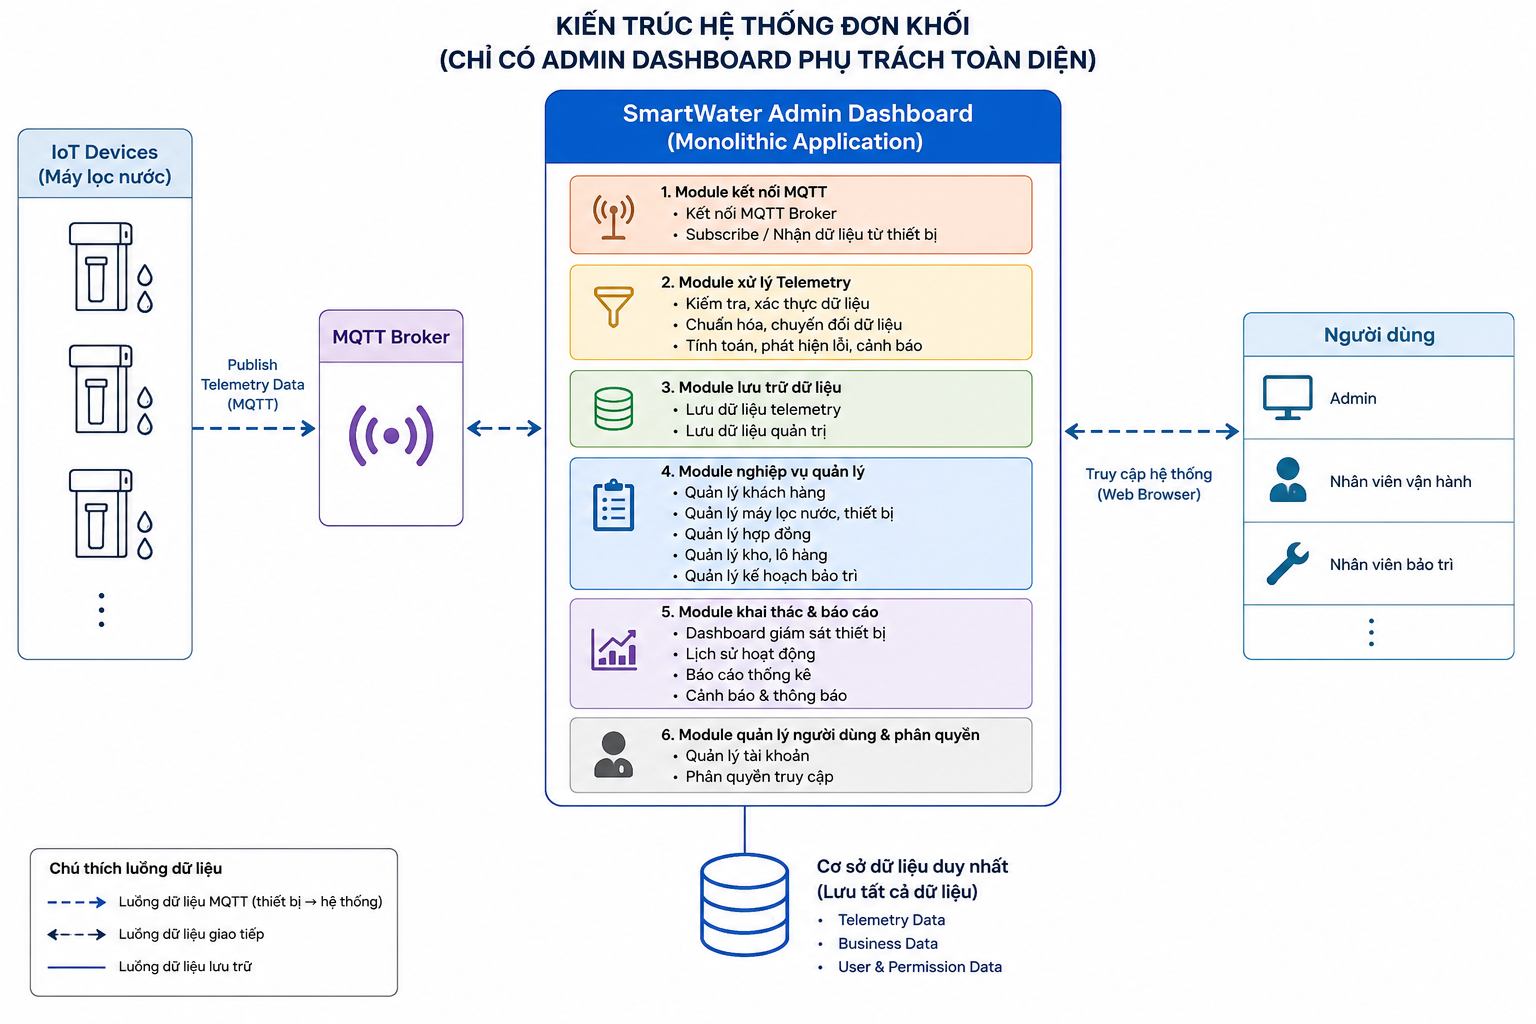
\includegraphics[width=0.8\textwidth]{include/image/he-thong-monolithic.png}
%     \caption{Kiến trúc hệ thống đơn khối}
%     \label{fig:monolithic}
% \end{figure}

Sau khi đánh giá, sinh viên lựa chọn kiến trúc lai giữa \textit{Layered Monolithic Web Application} và \textit{Event-Driven IoT Architecture}. SmartWater Admin là ứng dụng Laravel nguyên khối được tổ chức theo các tầng Route, Controller, Service, Eloquent Model, MySQL và Blade View. Luồng IoT được tách theo cơ chế hướng sự kiện, trong đó ESP32 gửi bản tin MQTT đến HiveMQ, Device Monitor tiếp nhận và chuẩn hóa dữ liệu trước khi lưu vào cơ sở dữ liệu MySQL dùng chung.

Kiến trúc được lựa chọn được trình bày trong Hình \ref{fig:software-architecture}.

\begin{figure}[H]
    \centering
    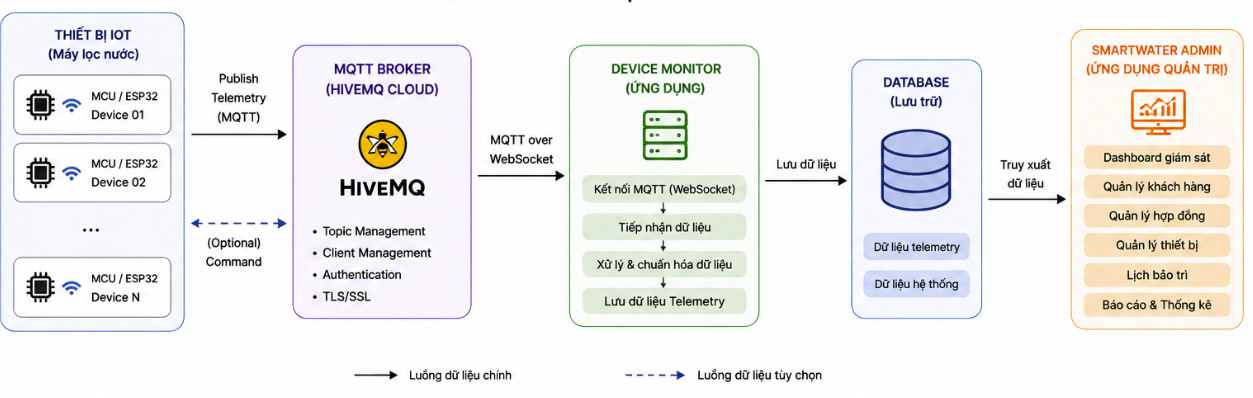
\includegraphics[width=0.8\linewidth]{include/image/IoT platform.png}
    \caption{Kiến trúc phần mềm của hệ thống SmartWater}
    \label{fig:software-architecture}
\end{figure}

Trong kiến trúc này, Device Monitor đóng vai trò là thành phần tích hợp giữa MQTT Broker và cơ sở dữ liệu, chịu trách nhiệm tiếp nhận, kiểm tra, chuẩn hóa và lưu trữ telemetry. SmartWater Admin khai thác dữ liệu đã xử lý thông qua các quan hệ nghiệp vụ trong MySQL mà không phải trực tiếp giao tiếp với thiết bị IoT.

Ngoài việc giảm sự phụ thuộc giữa các thành phần, kiến trúc này còn tạo ra một nguồn dữ liệu thống nhất để nhiều chức năng cùng khai thác. Trong tương lai, hệ thống có thể mở rộng thêm cảnh báo tự động, phân tích dữ liệu và dự đoán bảo trì mà không làm thay đổi luồng thu nhận telemetry hiện có.

% %%%%%%%%%%%%%%%%%%%%%%%%%%%%%%%%%%%%%%%%%%%%%
\tocsubsubsection{3.3 Thiết kế Device Monitor}
Sau khi hoàn thành thiết kế kiến trúc tổng thể của hệ thống, sinh viên tiếp tục thiết kế chi tiết ứng dụng Device Monitor. Đây là thành phần chịu trách nhiệm tiếp nhận dữ liệu telemetry từ các thiết bị IoT, xử lý dữ liệu trước khi lưu trữ và cung cấp nguồn dữ liệu thống nhất cho SmartWater Admin khai thác.

Device Monitor đảm nhiệm việc giao tiếp với MQTT Broker và xử lý dữ liệu telemetry. Việc tách riêng thành một ứng dụng độc lập giúp giảm sự phụ thuộc giữa lớp thu nhận dữ liệu và lớp nghiệp vụ, đồng thời tạo điều kiện mở rộng hệ thống khi số lượng thiết bị hoặc lưu lượng dữ liệu tăng lên.


\tocsubsubsubsection{3.3.1 Mục tiêu thiết kế}

Mục tiêu của Device Monitor là xây dựng một thành phần trung gian giữa các thiết bị IoT và hệ thống quản lý. Toàn bộ dữ liệu telemetry do các thiết bị gửi lên sẽ được Device Monitor tiếp nhận, kiểm tra, chuẩn hóa và lưu trữ trước khi được các ứng dụng khác sử dụng.

Kiến trúc này giúp SmartWater Admin không cần trực tiếp kết nối đến MQTT Broker hay xử lý các bản tin MQTT. Thay vào đó, SmartWater Admin chỉ khai thác dữ liệu đã được chuẩn hóa để phục vụ các nghiệp vụ quản lý, góp phần giảm sự phụ thuộc giữa các thành phần và nâng cao khả năng mở rộng của hệ thống.

\tocsubsubsubsection{3.3.2 Kiến trúc Device Monitor}
\paragraph{
Để đáp ứng các yêu cầu đã đặt ra, Device Monitor được thiết kế theo mô hình xử lý tuần tự (Pipeline Processing). Trong mô hình này, dữ liệu telemetry sẽ lần lượt đi qua các bước tiếp nhận, kiểm tra, xử lý và lưu trữ trước khi được cung cấp cho các ứng dụng khai thác.

Việc tổ chức theo mô hình pipeline giúp mỗi thành phần chỉ đảm nhiệm một nhiệm vụ cụ thể, từ đó giảm sự phụ thuộc giữa các module, thuận lợi cho việc bảo trì cũng như bổ sung thêm các bước xử lý trong tương lai.

Kiến trúc của Device Monitor bao gồm các thành phần sau:
}


\begin{itemize}
    \item \textbf{MQTT Subscriber}: Thiết lập kết nối đến HiveMQ Cloud thông qua MQTT over WebSocket và đăng ký lắng nghe các topic telemetry.

    \item \textbf{Message Receiver}: Tiếp nhận các bản tin MQTT từ Broker và chuyển dữ liệu sang các bước xử lý tiếp theo.

    \item \textbf{Data Validation}: Kiểm tra cấu trúc bản tin, xác thực các trường dữ liệu bắt buộc và loại bỏ các bản tin không hợp lệ.

    \item \textbf{Telemetry Processor}: Phân tích nội dung telemetry, chuẩn hóa dữ liệu và bổ sung các thông tin phục vụ lưu trữ.

    \item \textbf{Telemetry Database}: Lưu trữ dữ liệu telemetry đã được xử lý và cung cấp nguồn dữ liệu cho SmartWater Admin cũng như các ứng dụng khác.
\end{itemize}

Mô hình kiến trúc của Device Monitor được trình bày trong Hình \ref{fig:device-monitor-model}.

\begin{figure}[H]
    \centering
    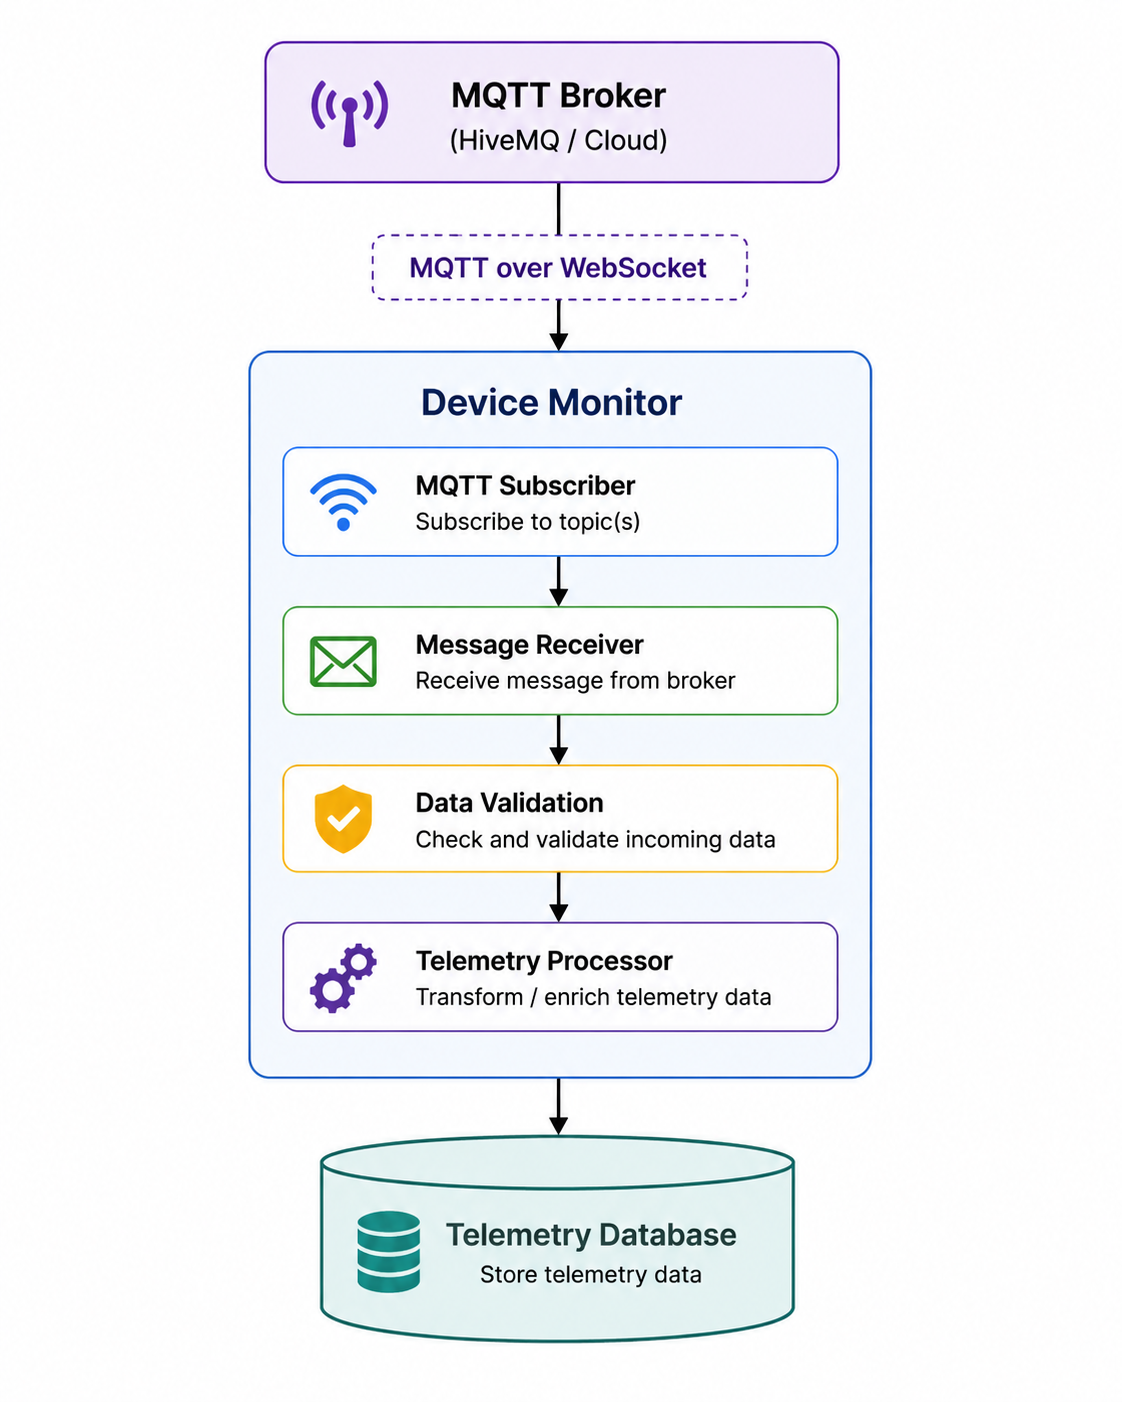
\includegraphics[width=0.5\linewidth]{include/image/Device-monitor.png}
    \caption{Kiến trúc phần mềm của Device Monitor}
    \label{fig:device-monitor-model}
\end{figure}

\tocsubsubsubsection{3.3.3 Luồng xử lý dữ liệu}

Quá trình xử lý dữ liệu của Device Monitor được thực hiện theo các bước sau:

\begin{enumerate}
    \item Thiết bị ESP32 gửi bản tin MQTT lên HiveMQ Cloud. Nội dung bản tin tối giản gồm mã MCU (\texttt{mcu\_id}), giá trị TDS (\texttt{tds}) và trạng thái cảnh báo (\texttt{alert}).

    \item MQTT Broker tiếp nhận bản tin và chuyển tiếp đến Device Monitor thông qua giao thức MQTT over WebSocket.

    \item MQTT Subscriber tiếp nhận bản tin và chuyển cho Message Receiver để bắt đầu quá trình xử lý.

    \item Data Validation kiểm tra cấu trúc dữ liệu, xác thực các trường thông tin bắt buộc và loại bỏ các bản tin không hợp lệ.

    \item Telemetry Processor phân tích nội dung telemetry, chuẩn hóa định dạng và bổ sung thời điểm tiếp nhận (\texttt{timestamp}) trước khi lưu trữ. Khóa chính của bản ghi được cơ sở dữ liệu tự động sinh.

    \item Dữ liệu sau khi được xử lý được lưu vào Telemetry Database, tạo thành nguồn dữ liệu thống nhất phục vụ các ứng dụng trong hệ thống.

    \item SmartWater Admin truy xuất telemetry thông qua \texttt{mcu\_id}. Từ MCU, hệ thống lần theo Product, Contract và Customer để hiển thị dữ liệu đúng máy lọc nước và khách hàng.
\end{enumerate}

Luồng xử lý này giúp toàn bộ quá trình chuẩn hóa dữ liệu được thực hiện tập trung tại Device Monitor. Nhờ đó, firmware trên thiết bị chỉ cần gửi các thông tin cần thiết, trong khi các ứng dụng phía sau luôn sử dụng cùng một cấu trúc dữ liệu đã được chuẩn hóa.

\tocsubsubsubsection{3.3.4 Chức năng của Device Monitor}

Dựa trên kiến trúc đã thiết kế, Device Monitor thực hiện các chức năng chính sau:

\begin{itemize}
    \item Thiết lập kết nối đến HiveMQ Cloud thông qua MQTT over WebSocket.
    \item Đăng ký lắng nghe các topic telemetry.
    \item Tiếp nhận bản tin MQTT từ các thiết bị IoT.
    \item Kiểm tra tính hợp lệ của bản tin và chuẩn hóa dữ liệu telemetry.
    \item Bổ sung thời điểm tiếp nhận dữ liệu trước khi lưu trữ.
    \item Lưu dữ liệu telemetry vào cơ sở dữ liệu.
    \item Cung cấp dữ liệu telemetry cho SmartWater Admin và các ứng dụng khác trong hệ thống.
\end{itemize}

\tocsubsubsubsection{3.3.5 Đánh giá thiết kế}
\paragraph{
Thiết kế Device Monitor đáp ứng mục tiêu xây dựng một thành phần chuyên trách cho việc thu nhận và xử lý dữ liệu telemetry từ các thiết bị IoT. Việc tách riêng Device Monitor khỏi SmartWater Admin giúp giảm sự phụ thuộc giữa quá trình giao tiếp với thiết bị và các nghiệp vụ quản lý, từ đó nâng cao khả năng bảo trì và phát triển hệ thống.

Bên cạnh đó, Device Monitor thực hiện việc kiểm tra, chuẩn hóa và lưu trữ dữ liệu tại một điểm tập trung, giúp đảm bảo tính nhất quán của dữ liệu telemetry trước khi được các ứng dụng khai thác. SmartWater Admin chỉ cần sử dụng dữ liệu đã được xử lý mà không cần quan tâm đến giao thức MQTT hay cấu trúc bản tin từ thiết bị.

Ngoài ra, kiến trúc này còn tạo nền tảng cho việc mở rộng hệ thống trong tương lai. Khi cần bổ sung các chức năng như cảnh báo thời gian thực, phân tích dữ liệu, dự đoán bảo trì hoặc các ứng dụng IoT khác, các thành phần mới có thể khai thác trực tiếp nguồn dữ liệu telemetry đã được chuẩn hóa mà không cần thay đổi quy trình thu nhận dữ liệu hiện có.
}
\tocsubsubsection{3.4 Định hướng mô phỏng SmartWater Admin}
\paragraph{
Sau khi hoàn thành thiết kế Device Monitor, sinh viên đề xuất mô phỏng SmartWater Admin nhằm minh họa cách khai thác dữ liệu phục vụ quản lý. Phần Website không thuộc phạm vi phụ trách chính của sinh viên và chưa có đầy đủ đặc tả nghiệp vụ chính thức từ khách hàng, do đó báo cáo chỉ trình bày định hướng ở mức tổng quan.

Khác với Device Monitor tập trung vào việc tiếp nhận và lưu trữ dữ liệu đo, SmartWater Admin được định hướng khai thác dữ liệu đã xử lý để phục vụ các chức năng quản lý. Việc tách biệt hai vai trò giúp giảm sự phụ thuộc giữa phần giám sát thiết bị và phần nghiệp vụ.
}
\tocsubsubsubsection{3.4.1 Mục tiêu thiết kế}
\paragraph{
Mô phỏng SmartWater Admin hướng đến minh họa khả năng tổ chức thông tin quản trị và khai thác dữ liệu vận hành ở mức tổng quan.
}
\begin{itemize}
    \item Minh họa giao diện tổng quan cho người quản trị.
    \item Thể hiện mối liên hệ giữa thiết bị, dữ liệu vận hành và thông tin nghiệp vụ.
    \item Tạo cơ sở trao đổi với khách hàng khi hoàn thiện đặc tả chức năng.
\end{itemize}

Trong định hướng này, Website chỉ khai thác dữ liệu đã được xử lý và lưu trữ, không trực tiếp giao tiếp với thiết bị hoặc nền tảng truyền thông.

\tocsubsubsubsection{3.4.2 Kiến trúc SmartWater Admin}
\paragraph{
Kiến trúc mô phỏng gồm lớp giao diện quản trị, lớp xử lý nghiệp vụ và lớp khai thác dữ liệu đã lưu trữ. Các thành phần được mô tả nhằm làm rõ luồng thông tin tổng quát từ dữ liệu vận hành đến các màn hình phục vụ người quản trị; thiết kế chi tiết và cách triển khai nội bộ không được công bố trong báo cáo.
}

\tocsubsubsubsection{3.4.3 Các module nghiệp vụ}

Các nhóm chức năng mô phỏng gồm tổng quan vận hành, thông tin thiết bị, khách hàng, hợp đồng và các dữ liệu phục vụ công tác quản lý. Phạm vi và quy trình chi tiết của từng nhóm sẽ được xác định khi có đặc tả chính thức từ khách hàng.

\tocsubsubsubsection{3.4.4 Luồng xử lý nghiệp vụ}

Luồng nghiệp vụ được mô phỏng theo hướng người quản trị truy cập giao diện, xem dữ liệu vận hành đã được lưu trữ và sử dụng thông tin tổng hợp để theo dõi thiết bị. Cách tổ chức này giúp phần quản trị tập trung vào khai thác thông tin thay vì trực tiếp xử lý kết nối với thiết bị IoT.

\tocsubsubsubsection{3.4.5 Đánh giá thiết kế}
\paragraph{
Thiết kế ở mức mô phỏng đáp ứng mục tiêu minh họa cách liên kết dữ liệu vận hành với các nhu cầu quản lý cơ bản. Khi yêu cầu khách hàng được làm rõ, các chức năng, giao diện và tiêu chí nghiệm thu cần được phân tích, thiết kế và kiểm thử riêng trước khi triển khai chính thức.
}

\tocsubsubsection{3.5 Định hướng tổ chức dữ liệu}
\paragraph{
Cơ sở dữ liệu được tổ chức để lưu trữ dữ liệu đo từ thiết bị và hỗ trợ liên kết với các thông tin quản lý cần thiết. Các cấu trúc bảng, quan hệ chi tiết, quy tắc truy cập và thông tin cấu hình thuộc phạm vi nội bộ của doanh nghiệp nên không được trình bày trong báo cáo.
}

Dữ liệu được lưu trữ có cấu trúc để phục vụ việc tra cứu lịch sử đo, theo dõi thiết bị và cung cấp thông tin cho các màn hình giám sát hoặc quản lý ở mức phù hợp.

\tocsubsubsection{3.6 Lựa chọn công nghệ}
\paragraph{
Sau khi hoàn thành quá trình phân tích yêu cầu và thiết kế kiến trúc phần mềm, sinh viên tiến hành khảo sát và lựa chọn các công nghệ phù hợp để triển khai hệ thống SmartWater. Việc lựa chọn được thực hiện dựa trên các tiêu chí như khả năng đáp ứng yêu cầu của hệ thống, tính ổn định, khả năng mở rộng, mức độ phổ biến của cộng đồng và sự phù hợp với định hướng phát triển của dự án.

Các công nghệ được lựa chọn bao gồm MQTT kết hợp với HiveMQ Cloud cho quá trình truyền nhận dữ liệu IoT, PHP và Laravel để phát triển các ứng dụng web, cùng với MySQL làm hệ quản trị cơ sở dữ liệu.
}
\tocsubsubsubsection{3.6.1 MQTT và HiveMQ}
\paragraph{
Một trong những yêu cầu quan trọng của hệ thống SmartWater là tiếp nhận dữ liệu telemetry từ nhiều thiết bị IoT hoạt động đồng thời. Vì vậy, hệ thống cần một cơ chế truyền nhận dữ liệu có độ trễ thấp, hỗ trợ nhiều thiết bị kết nối cùng lúc và dễ dàng mở rộng khi số lượng thiết bị tăng lên.

Sau quá trình khảo sát, sinh viên lựa chọn giao thức MQTT (Message Queuing Telemetry Transport) kết hợp với HiveMQ Cloud để xây dựng hệ thống truyền nhận dữ liệu.

MQTT hoạt động theo mô hình Publish/Subscribe, trong đó các thiết bị IoT đóng vai trò Publisher gửi dữ liệu telemetry lên MQTT Broker, còn Device Monitor đóng vai trò Subscriber tiếp nhận các bản tin thông qua MQTT over WebSocket. Cơ chế này giúp tách biệt hoàn toàn giữa thiết bị và ứng dụng xử lý dữ liệu, giảm sự phụ thuộc giữa các thành phần và cho phép nhiều ứng dụng có thể cùng khai thác dữ liệu từ Broker.

HiveMQ Cloud được lựa chọn làm MQTT Broker do cung cấp dịch vụ trên nền tảng đám mây, hỗ trợ kết nối bảo mật bằng TLS, quản lý topic linh hoạt và dễ dàng tích hợp với các ứng dụng web. Việc sử dụng HiveMQ Cloud giúp giảm thời gian triển khai hạ tầng MQTT, đồng thời thuận lợi cho quá trình thử nghiệm và phát triển hệ thống.
}
\tocsubsubsubsection{3.6.2 PHP}
\paragraph{
Do hệ thống SmartWater bao gồm các ứng dụng web phục vụ quản lý và giám sát thiết bị, sinh viên lựa chọn PHP làm ngôn ngữ lập trình chính trong quá trình phát triển.

PHP là ngôn ngữ lập trình phía máy chủ (Server-side Scripting Language) được sử dụng rộng rãi trong các hệ thống web. Ngôn ngữ này có ưu điểm là dễ triển khai, có cộng đồng phát triển lớn, nhiều thư viện hỗ trợ và tương thích với hầu hết các hệ quản trị cơ sở dữ liệu phổ biến.

Bên cạnh đó, PHP phù hợp với cả Device Monitor và SmartWater Admin. Device Monitor sử dụng PHP cho API tiếp nhận và lưu telemetry, trong khi SmartWater Admin sử dụng Laravel để tổ chức các tầng nghiệp vụ và giao diện quản trị.
}


\tocsubsubsubsection{3.6.3 Laravel}
\paragraph{
Laravel được lựa chọn làm framework phát triển SmartWater Admin. Device Monitor là ứng dụng tích hợp MQTT độc lập và không được tổ chức như một ứng dụng Laravel.

Laravel là framework mã nguồn mở được phát triển trên nền tảng PHP theo mô hình MVC (Model--View--Controller). Framework cung cấp nhiều thành phần hỗ trợ như Routing, Middleware, ORM Eloquent, Migration, Authentication và Dependency Injection, giúp tổ chức mã nguồn rõ ràng và giảm khối lượng công việc trong quá trình phát triển.

Việc sử dụng Laravel giúp hiện thực chuỗi Route, Controller, Service, Eloquent Model và Blade View, phù hợp với kiến trúc nguyên khối phân lớp. Migration và Eloquent ORM đồng thời giúp các truy vấn tuân theo cấu trúc bảng và quan hệ dữ liệu đã chuẩn hóa.
}
\tocsubsubsubsection{3.6.4 ASP.NET Core}
\paragraph{
Trong giai đoạn khảo sát công nghệ, sinh viên tiến hành tìm hiểu ASP.NET Core như một phương án để phát triển các ứng dụng phía máy chủ. ASP.NET Core là framework mã nguồn mở do Microsoft phát triển, hỗ trợ xây dựng các ứng dụng web, RESTful API và các dịch vụ backend với hiệu năng cao.

Framework này cung cấp nhiều tính năng hỗ trợ phát triển phần mềm như Dependency Injection, Middleware, Logging, Authentication và khả năng triển khai đa nền tảng trên Windows, Linux và macOS. Bên cạnh đó, ASP.NET Core có khả năng xử lý đồng thời nhiều yêu cầu, phù hợp với các hệ thống có lưu lượng truy cập lớn và yêu cầu khả năng mở rộng cao.

Qua quá trình nghiên cứu, sinh viên nhận thấy ASP.NET Core là một lựa chọn phù hợp đối với các hệ thống backend và các dịch vụ xử lý dữ liệu. Tuy nhiên, sau khi đánh giá yêu cầu của dự án, nhóm quyết định lựa chọn PHP kết hợp với Laravel nhằm đảm bảo tính thống nhất giữa các thành phần của hệ thống và phù hợp với môi trường phát triển tại doanh nghiệp.
}

\tocsubsubsubsection{3.6.5 MySQL}
\paragraph{
Hệ thống SmartWater cần lưu trữ đồng thời dữ liệu telemetry từ các thiết bị IoT và dữ liệu nghiệp vụ của hệ thống quản lý. Do đó, sinh viên lựa chọn MySQL làm hệ quản trị cơ sở dữ liệu cho dự án.

MySQL là hệ quản trị cơ sở dữ liệu quan hệ (Relational Database Management System -- RDBMS) được sử dụng phổ biến trong các ứng dụng web. Hệ quản trị này hỗ trợ ngôn ngữ SQL, quản lý dữ liệu theo mô hình quan hệ và đảm bảo tính toàn vẹn dữ liệu thông qua các ràng buộc và cơ chế giao dịch.

Trong hệ thống SmartWater, MySQL \texttt{smartwater\_database} là nguồn dữ liệu dùng chung cho Device Monitor và SmartWater Admin. Dữ liệu nghiệp vụ được liên kết theo chuỗi Customer, Contract, Product, Device và MCU; bảng telemetry lưu định danh MCU bằng \texttt{mcu\_id}. Cấu trúc này giúp SmartWater Admin truy xuất telemetry của đúng MCU đang gắn với Product trong hợp đồng của khách hàng.
}
